% generated by Plantuml 1.2024.0       
\definecolor{plantucolor0000}{RGB}{0,0,0}
\definecolor{plantucolor0001}{RGB}{241,241,241}
\definecolor{plantucolor0002}{RGB}{24,24,24}
\definecolor{plantucolor0003}{RGB}{169,220,223}
\definecolor{plantucolor0004}{RGB}{132,190,132}
\definecolor{plantucolor0005}{RGB}{3,128,72}
\definecolor{plantucolor0006}{RGB}{180,167,229}
\definecolor{plantucolor0007}{RGB}{173,209,178}
\definecolor{plantucolor0008}{RGB}{242,77,92}
\definecolor{plantucolor0009}{RGB}{200,41,48}
\definecolor{plantucolor0010}{RGB}{254,255,221}
\scalebox{0.6}{
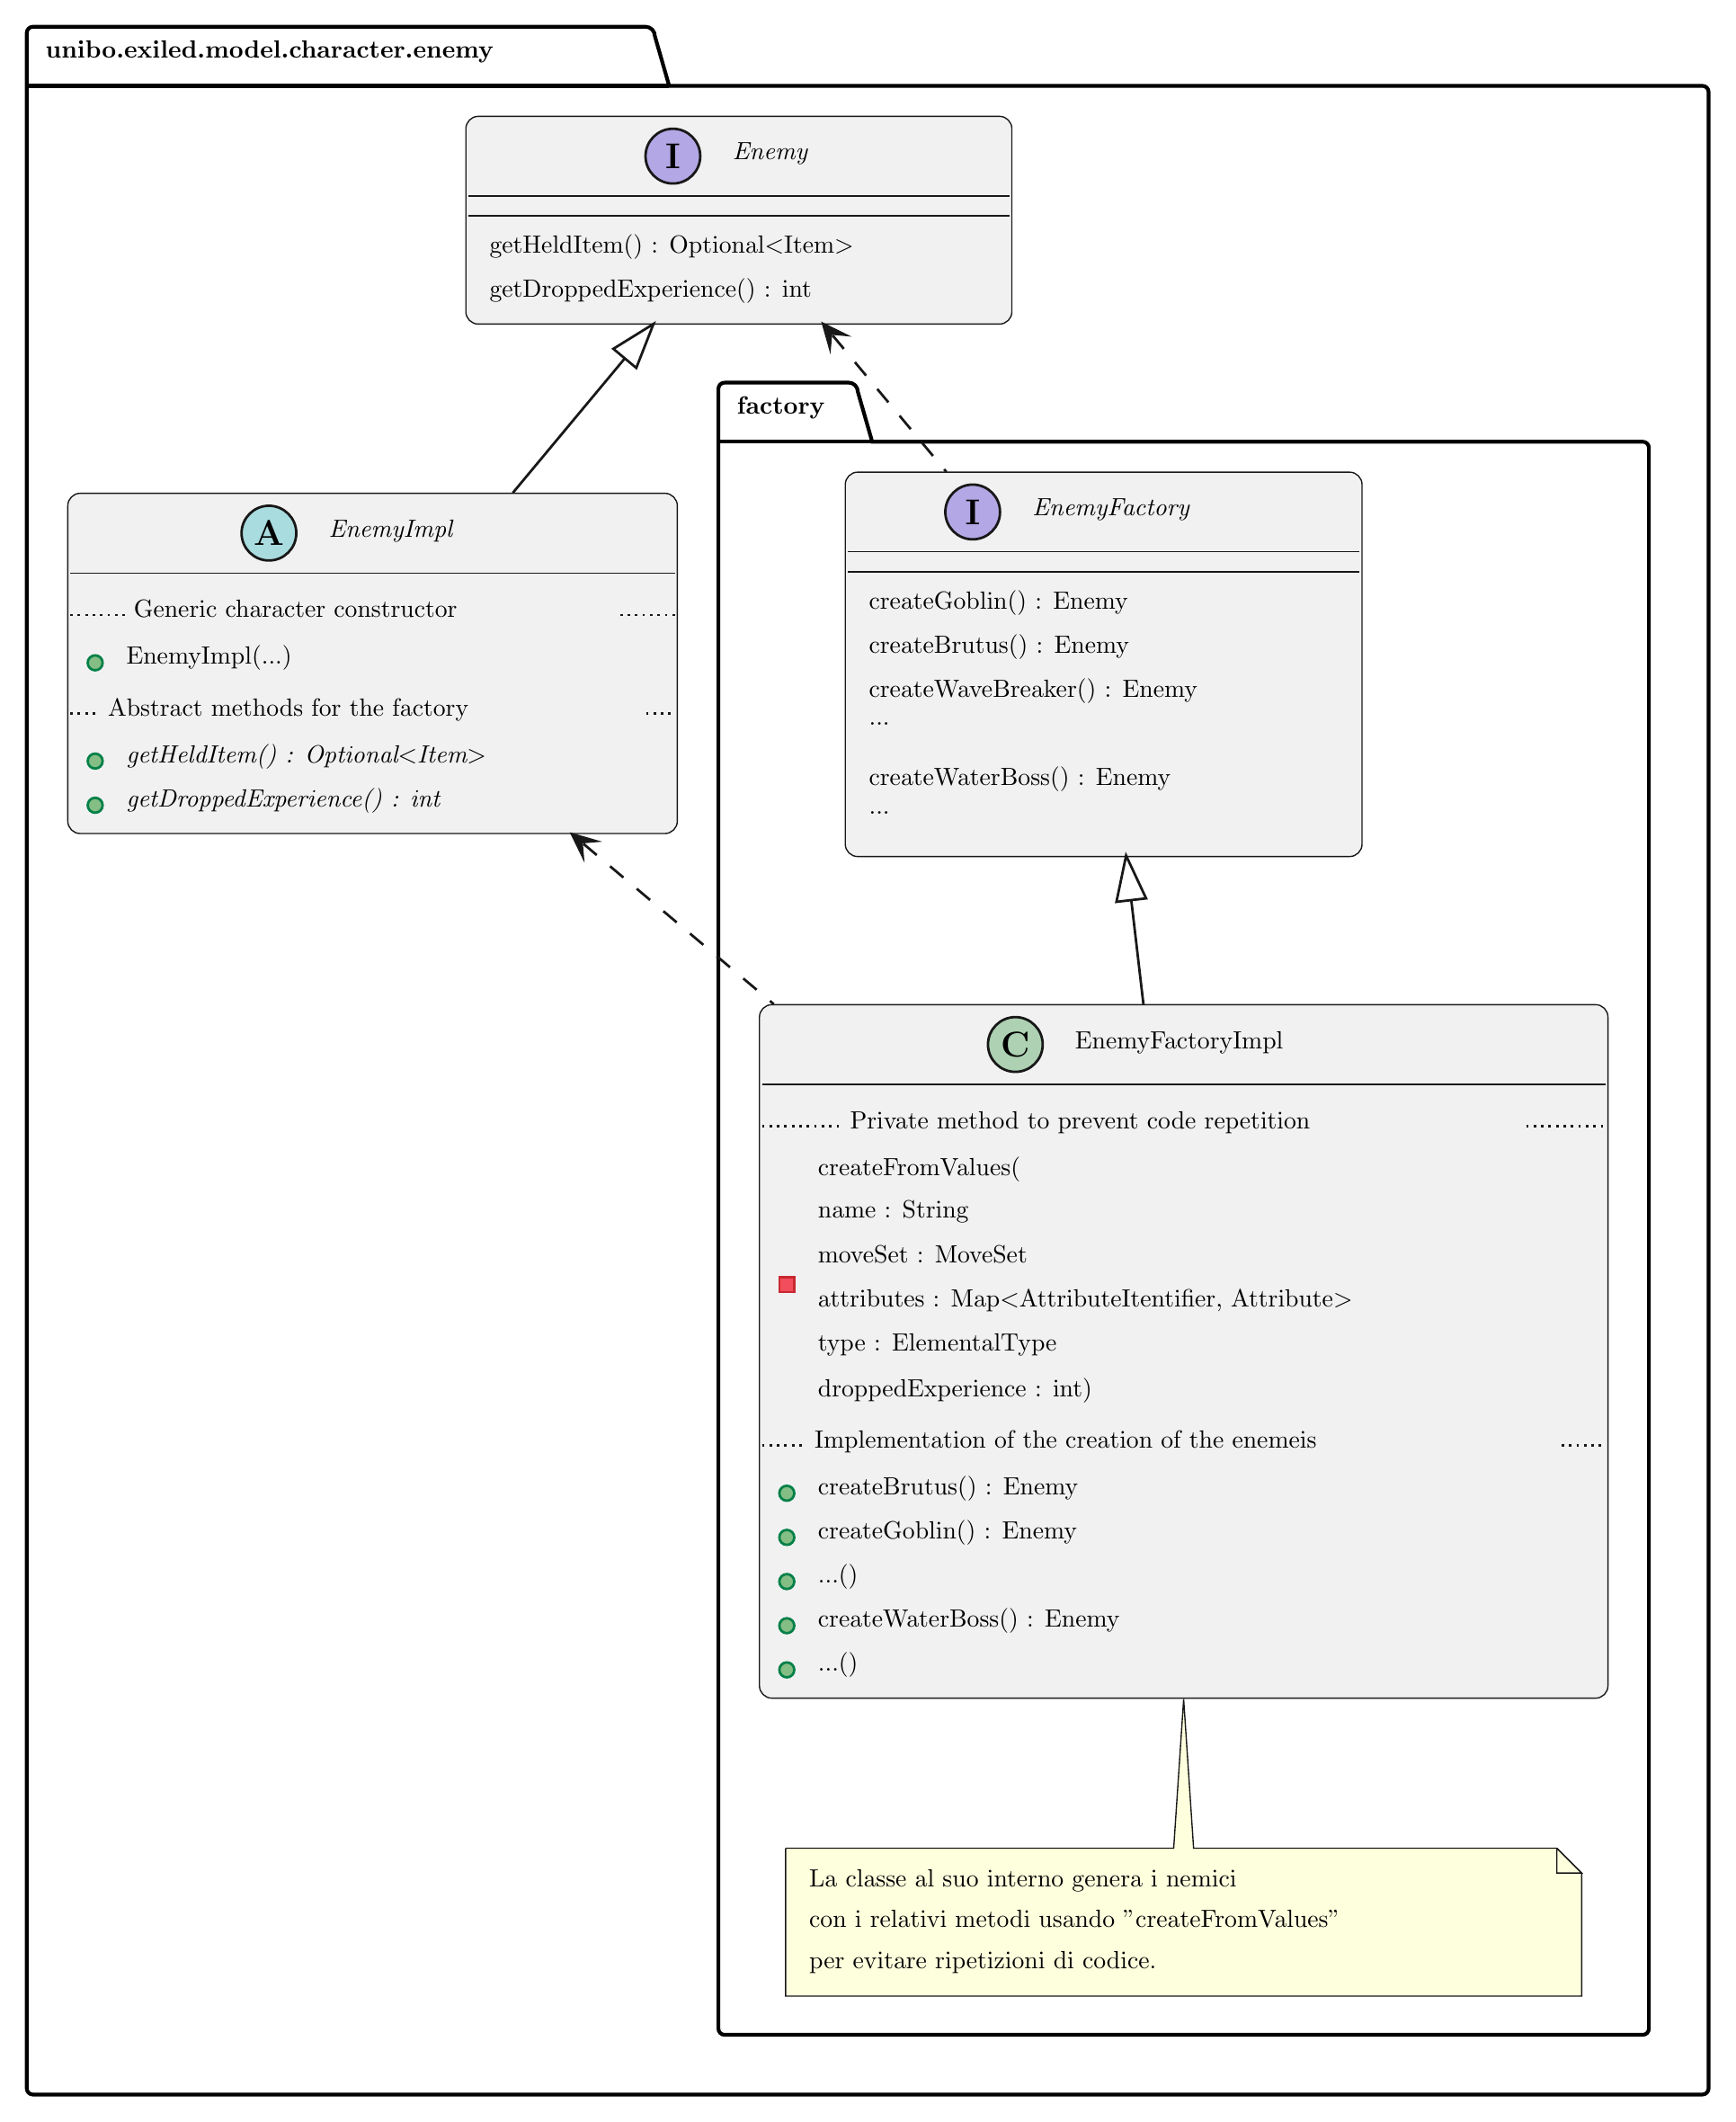
\begin{tikzpicture}[yscale=-1
,pstyle0/.style={color=black,line width=1.5pt}
,pstyle1/.style={color=plantucolor0002,fill=plantucolor0001,line width=0.5pt}
,pstyle3/.style={color=plantucolor0002,line width=0.5pt}
,pstyle4/.style={color=plantucolor0005,fill=plantucolor0004,line width=1.0pt}
,pstyle5/.style={color=plantucolor0002,line width=1.0pt,dash pattern=on 1.0pt off 2.0pt}
,pstyle6/.style={color=plantucolor0002,fill=plantucolor0006,line width=1.0pt}
,pstyle9/.style={color=plantucolor0002,fill=plantucolor0010,line width=0.5pt}
,pstyle10/.style={color=plantucolor0002,line width=1.0pt}
,pstyle11/.style={color=plantucolor0002,line width=1.0pt,dash pattern=on 7.0pt off 7.0pt}
,pstyle12/.style={color=plantucolor0002,fill=plantucolor0002,line width=1.0pt}
]
\draw[pstyle0] (8.5pt,6pt) -- (254.7108pt,6pt) arc(270:360:3.75pt)  -- (264.2108pt,29.7461pt) -- (679.5pt,29.7461pt) arc(270:360:2.5pt)  -- (682pt,834.5pt) arc(0:90:2.5pt)  -- (8.5pt,837pt) arc(90:180:2.5pt)  -- (6pt,8.5pt) arc(180:270:2.5pt) ;
\draw[pstyle0] (6pt,29.7461pt) -- (264.2108pt,29.7461pt);
\node at (10pt,8pt)[below right,color=black]{\textbf{unibo.exiled.model.character.enemy}};
\draw[pstyle0] (286.5pt,149pt) -- (336.3093pt,149pt) arc(270:360:3.75pt)  -- (345.8093pt,172.7461pt) -- (655.5pt,172.7461pt) arc(270:360:2.5pt)  -- (658pt,810.5pt) arc(0:90:2.5pt)  -- (286.5pt,813pt) arc(90:180:2.5pt)  -- (284pt,151.5pt) arc(180:270:2.5pt) ;
\draw[pstyle0] (284pt,172.7461pt) -- (345.8093pt,172.7461pt);
\node at (288pt,151pt)[below right,color=black]{\textbf{factory}};
\draw[pstyle1] (22.5pt,198.5pt) arc (180:270:5pt) -- (27.5pt,193.5pt) -- (262.4882pt,193.5pt) arc (270:360:5pt) -- (267.4882pt,198.5pt) -- (267.4882pt,325.2305pt) arc (0:90:5pt) -- (262.4882pt,330.2305pt) -- (27.5pt,330.2305pt) arc (90:180:5pt) -- (22.5pt,325.2305pt) -- cycle;
\draw[color=plantucolor0002,fill=plantucolor0003,line width=1.0pt] (103.3441pt,209.5pt) ellipse (11pt and 11pt);
\node at (103.3441pt,209.5pt)[]{\textbf{\Large A}};
\node at (123.8441pt,200.627pt)[below right,color=black]{\textit{EnemyImpl}};
\draw[pstyle3] (23.5pt,225.5pt) -- (266.4882pt,225.5pt);
\draw[pstyle4] (33.5pt,261.6191pt) ellipse (3pt and 3pt);
\node at (42.5pt,251.2461pt)[below right,color=black]{EnemyImpl(...)};
\draw[pstyle5] (23.5pt,242.373pt) -- (45.5052pt,242.373pt);
\node at (45.5052pt,233pt)[below right,color=black]{Generic character constructor};
\draw[pstyle5] (244.483pt,242.373pt) -- (266.4882pt,242.373pt);
\draw[pstyle4] (33.5pt,301.1113pt) ellipse (3pt and 3pt);
\node at (42.5pt,290.7383pt)[below right,color=black]{\textit{getHeldItem() : Optional\textless Item\textgreater }};
\draw[pstyle4] (33.5pt,318.8574pt) ellipse (3pt and 3pt);
\node at (42.5pt,308.4844pt)[below right,color=black]{\textit{getDroppedExperience() : int}};
\draw[pstyle5] (23.5pt,281.8652pt) -- (35.1043pt,281.8652pt);
\node at (35.1043pt,272.4922pt)[below right,color=black]{Abstract methods for the factory};
\draw[pstyle5] (254.884pt,281.8652pt) -- (266.4882pt,281.8652pt);
\draw[pstyle1] (182.5pt,47pt) arc (180:270:5pt) -- (187.5pt,42pt) -- (396.9652pt,42pt) arc (270:360:5pt) -- (401.9652pt,47pt) -- (401.9652pt,120.4922pt) arc (0:90:5pt) -- (396.9652pt,125.4922pt) -- (187.5pt,125.4922pt) arc (90:180:5pt) -- (182.5pt,120.4922pt) -- cycle;
\draw[pstyle6] (265.7089pt,58pt) ellipse (11pt and 11pt);
\node at (265.7089pt,58pt)[]{\textbf{\Large I}};
\node at (286.2089pt,49.127pt)[below right,color=black]{\textit{Enemy}};
\draw[pstyle3] (183.5pt,74pt) -- (400.9652pt,74pt);
\draw[pstyle3] (183.5pt,82pt) -- (400.9652pt,82pt);
\node at (188.5pt,86pt)[below right,color=black]{getHeldItem() : Optional\textless Item\textgreater };
\node at (188.5pt,103.7461pt)[below right,color=black]{getDroppedExperience() : int};
\draw[pstyle1] (335pt,190pt) arc (180:270:5pt) -- (340pt,185pt) -- (537.6994pt,185pt) arc (270:360:5pt) -- (542.6994pt,190pt) -- (542.6994pt,334.4766pt) arc (0:90:5pt) -- (537.6994pt,339.4766pt) -- (340pt,339.4766pt) arc (90:180:5pt) -- (335pt,334.4766pt) -- cycle;
\draw[pstyle6] (386.2046pt,201pt) ellipse (11pt and 11pt);
\node at (386.2046pt,201pt)[]{\textbf{\Large I}};
\node at (406.7046pt,192.127pt)[below right,color=black]{\textit{EnemyFactory}};
\draw[pstyle3] (336pt,217pt) -- (541.6994pt,217pt);
\draw[pstyle3] (336pt,225pt) -- (541.6994pt,225pt);
\node at (341pt,229pt)[below right,color=black]{createGoblin() : Enemy};
\node at (341pt,246.7461pt)[below right,color=black]{createBrutus() : Enemy};
\node at (341pt,264.4922pt)[below right,color=black]{createWaveBreaker() : Enemy};
\node at (341pt,282.2383pt)[below right,color=black]{...};
\node at (341pt,299.9844pt)[below right,color=black]{createWaterBoss() : Enemy};
\node at (341pt,317.7305pt)[below right,color=black]{...};
\draw[pstyle1] (300.5pt,404pt) arc (180:270:5pt) -- (305.5pt,399pt) -- (636.5496pt,399pt) arc (270:360:5pt) -- (641.5496pt,404pt) -- (641.5496pt,672.6992pt) arc (0:90:5pt) -- (636.5496pt,677.6992pt) -- (305.5pt,677.6992pt) arc (90:180:5pt) -- (300.5pt,672.6992pt) -- cycle;
\draw[color=plantucolor0002,fill=plantucolor0007,line width=1.0pt] (403.3565pt,415pt) ellipse (11pt and 11pt);
\node at (403.3565pt,415pt)[]{\textbf{\Large C}};
\node at (423.8565pt,406.127pt)[below right,color=black]{EnemyFactoryImpl};
\draw[pstyle3] (301.5pt,431pt) -- (640.5496pt,431pt);
\draw[color=plantucolor0009,fill=plantucolor0008,line width=1.0pt] (308.5pt,508.4844pt) rectangle (314.5pt,514.4844pt);
\node at (320.5pt,456.7461pt)[below right,color=black]{createFromValues( };
\node at (320.5pt,474.4922pt)[below right,color=black]{ name : String };
\node at (320.5pt,492.2383pt)[below right,color=black]{ moveSet : MoveSet };
\node at (320.5pt,509.9844pt)[below right,color=black]{ attributes : Map\textless AttributeItentifier, Attribute\textgreater  };
\node at (320.5pt,527.7305pt)[below right,color=black]{ type : ElementalType };
\node at (320.5pt,545.4766pt)[below right,color=black]{ droppedExperience : int)};
\draw[pstyle5] (301.5pt,447.873pt) -- (333.3879pt,447.873pt);
\node at (333.3879pt,438.5pt)[below right,color=black]{Private method to prevent code repetition};
\draw[pstyle5] (608.6617pt,447.873pt) -- (640.5496pt,447.873pt);
\draw[pstyle4] (311.5pt,595.3418pt) ellipse (3pt and 3pt);
\node at (320.5pt,584.9688pt)[below right,color=black]{createBrutus() : Enemy};
\draw[pstyle4] (311.5pt,613.0879pt) ellipse (3pt and 3pt);
\node at (320.5pt,602.7148pt)[below right,color=black]{createGoblin() : Enemy};
\draw[pstyle4] (311.5pt,630.834pt) ellipse (3pt and 3pt);
\node at (320.5pt,620.4609pt)[below right,color=black]{...()};
\draw[pstyle4] (311.5pt,648.5801pt) ellipse (3pt and 3pt);
\node at (320.5pt,638.207pt)[below right,color=black]{createWaterBoss() : Enemy};
\draw[pstyle4] (311.5pt,666.3262pt) ellipse (3pt and 3pt);
\node at (320.5pt,655.9531pt)[below right,color=black]{...()};
\draw[pstyle5] (301.5pt,576.0957pt) -- (319.1692pt,576.0957pt);
\node at (319.1692pt,566.7227pt)[below right,color=black]{Implementation of the creation of the enemeis};
\draw[pstyle5] (622.8804pt,576.0957pt) -- (640.5496pt,576.0957pt);
\draw[pstyle9] (311pt,738pt) -- (311pt,797.4355pt) -- (311pt,797.4355pt) -- (630.9916pt,797.4355pt) -- (630.9916pt,797.4355pt) -- (630.9916pt,748pt) -- (620.9916pt,738pt) -- (475pt,738pt) -- (471pt,678.09pt) -- (467pt,738pt) -- (311pt,738pt) -- (311pt,738pt);
\draw[pstyle9] (620.9916pt,738pt) -- (620.9916pt,748pt) -- (630.9916pt,748pt) -- (620.9916pt,738pt);
\node at (317pt,743pt)[below right,color=black]{La classe al suo interno genera i nemici };
\node at (317pt,759.4785pt)[below right,color=black]{ con i relativi metodi usando "createFromValues" };
\node at (317pt,775.957pt)[below right,color=black]{ per evitare ripetizioni di codice.};
\draw[pstyle10] (246.3867pt,139.268pt) ..controls (229.5867pt,159.428pt) and (220.42pt,170.44pt) .. (201.36pt,193.33pt);
\draw[pstyle10] (257.91pt,125.44pt) -- (241.7774pt,135.4269pt) -- (250.996pt,143.1091pt) -- (257.91pt,125.44pt) -- cycle;
\draw[pstyle11] (329.9301pt,130.0502pt) ..controls (344.6901pt,147.7702pt) and (358.62pt,164.49pt) .. (375.65pt,184.93pt);
\draw[pstyle12] (326.09pt,125.44pt) -- (328.7767pt,134.9153pt) -- (329.2901pt,129.2818pt) -- (334.9236pt,129.7952pt) -- (326.09pt,125.44pt) -- cycle;
\draw[pstyle10] (449.9514pt,356.9793pt) ..controls (452.1214pt,375.6193pt) and (452.44pt,378.28pt) .. (454.84pt,398.85pt);
\draw[pstyle10] (447.87pt,339.1pt) -- (443.9917pt,357.6731pt) -- (455.9112pt,356.2854pt) -- (447.87pt,339.1pt) -- cycle;
\draw[pstyle11] (229.7587pt,334.3657pt) ..controls (254.4487pt,355.1657pt) and (278.02pt,375pt) .. (306.24pt,398.77pt);
\draw[pstyle12] (225.17pt,330.5pt) -- (229.4759pt,339.3577pt) -- (228.9939pt,333.7214pt) -- (234.6302pt,333.2395pt) -- (225.17pt,330.5pt) -- cycle;
\end{tikzpicture}
}
